\section{Resultate}
Bei den Resultaten handelt es sich um die Datenstrukturen, welche in Kapitel \ref{sec:implementation} beschreiben sind.
Bei Erweiterung ``\_impr'' handelt es sich um eine Verbesserte Version vie in Kapitel \ref{sec:mem} beschrieben.
Bei Datenstrukturen mit der Erweiterung ``\_mem'' ist ein Memorymanagement implementiert (siehe \ref{sec:mem}).
Alle Benchmarks wurden auf den TU Nebula Maschine ausgeführt. Aufgrund der beschrankten Rechenzeit auf dieser Maschine,
wurden die Test nur 10 Mal wiederholt. Die Folgenden Abbildungen zeigen jeweils den Mittelwert aller Wiederholungen.

\subsection{Laufzeit mit 64 Cores}

\subsubsection{Schreibvorgang}
\begin{figure}[ht!]
	\centering
	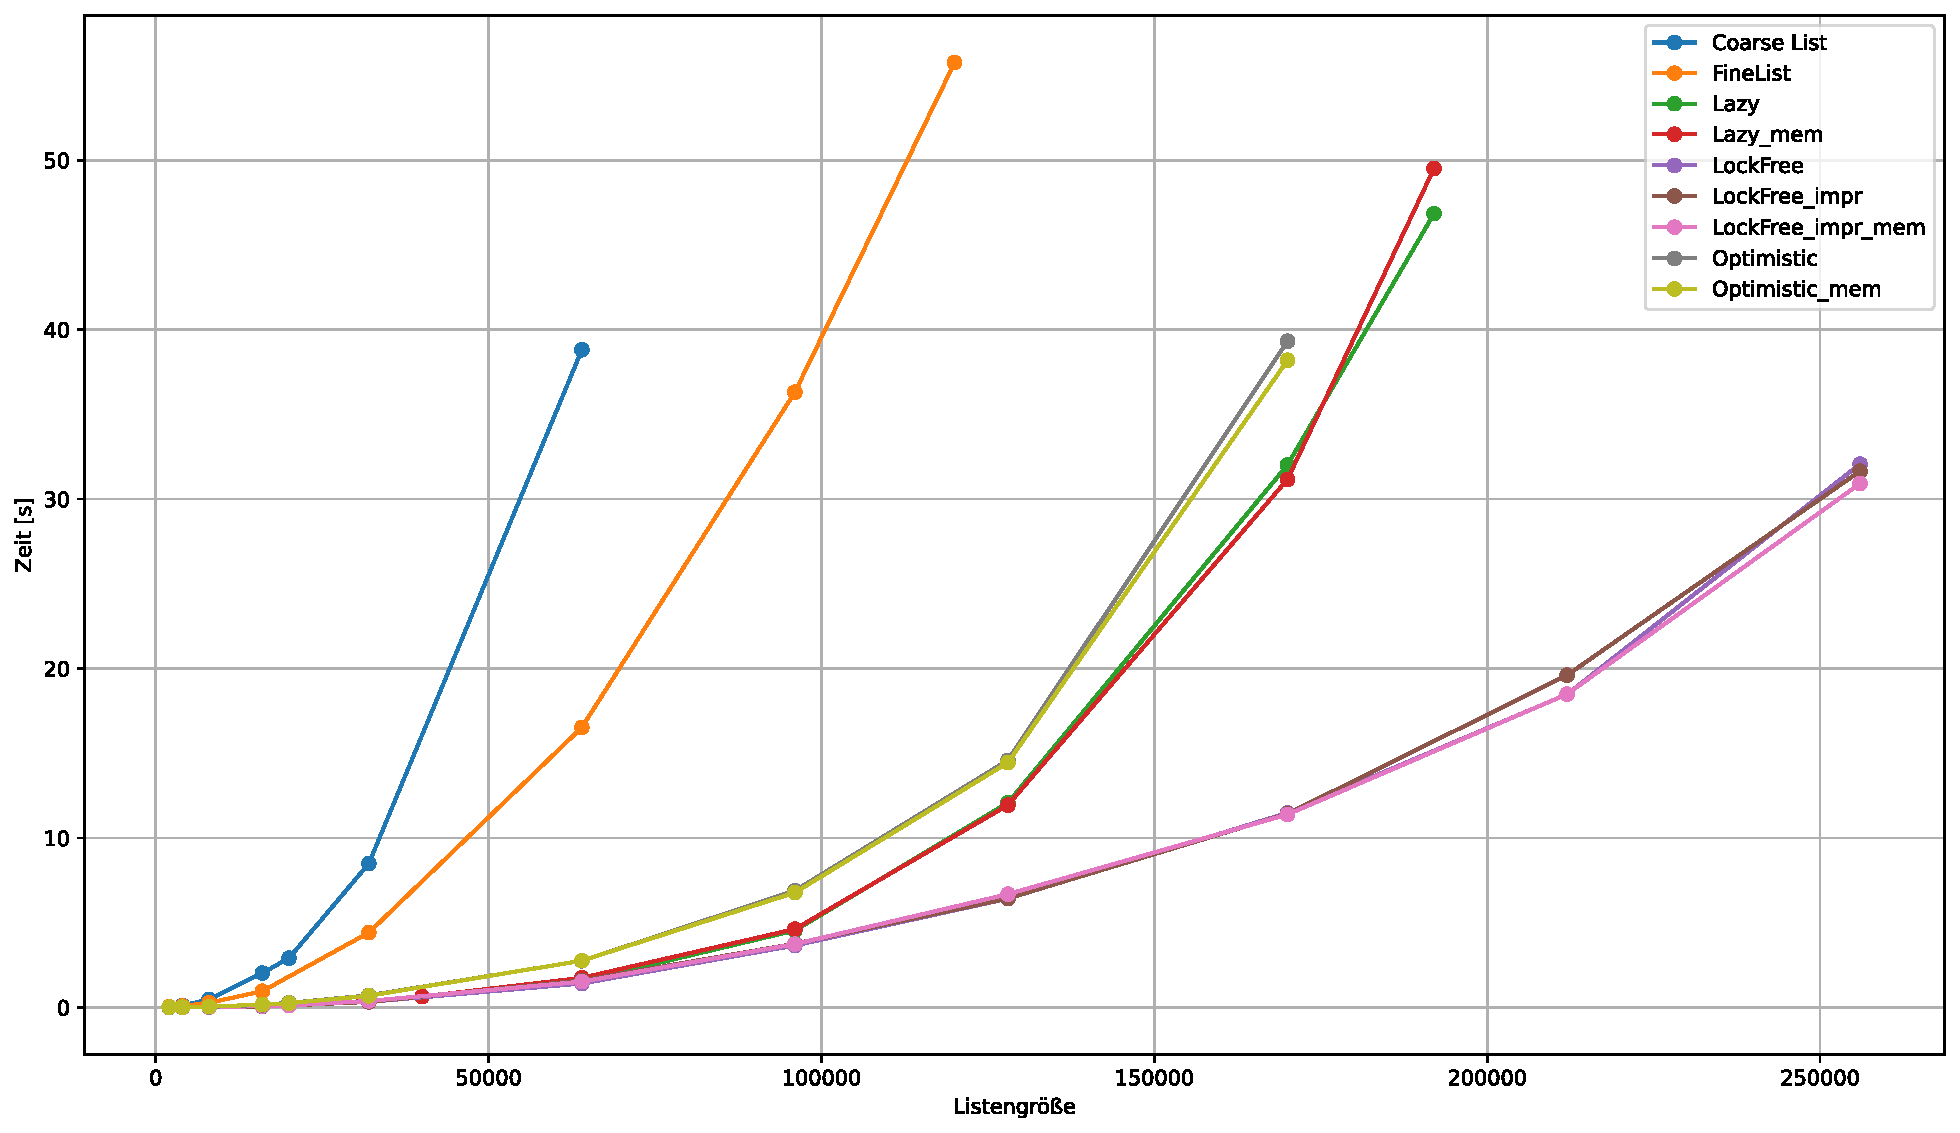
\includegraphics[width=1.0\linewidth]{./plots_pdf/write_time} 
	\caption{Laufzeit des Schreibvorganges}
	\label{fig:write_time} 
\end{figure}
Die Abbildung \ref{fig:write_time} zeigt die benötigte Laufzeit in Sekunden für das Einfügen von Elementen in eine leere Liste.
Dabei ist auf der X-Achse die Anzahl der eingefügten Elemente zu sehen. 
Das \textit{List-based set with coarse-grained locks} ist dabei am Langsamsten, da nur jeweils ein Node gleichzeitig 
Zugriff auf die Liste hat. 

\subsubsection{Gemischter Zugriff}
\begin{figure}[ht!]
	\centering
	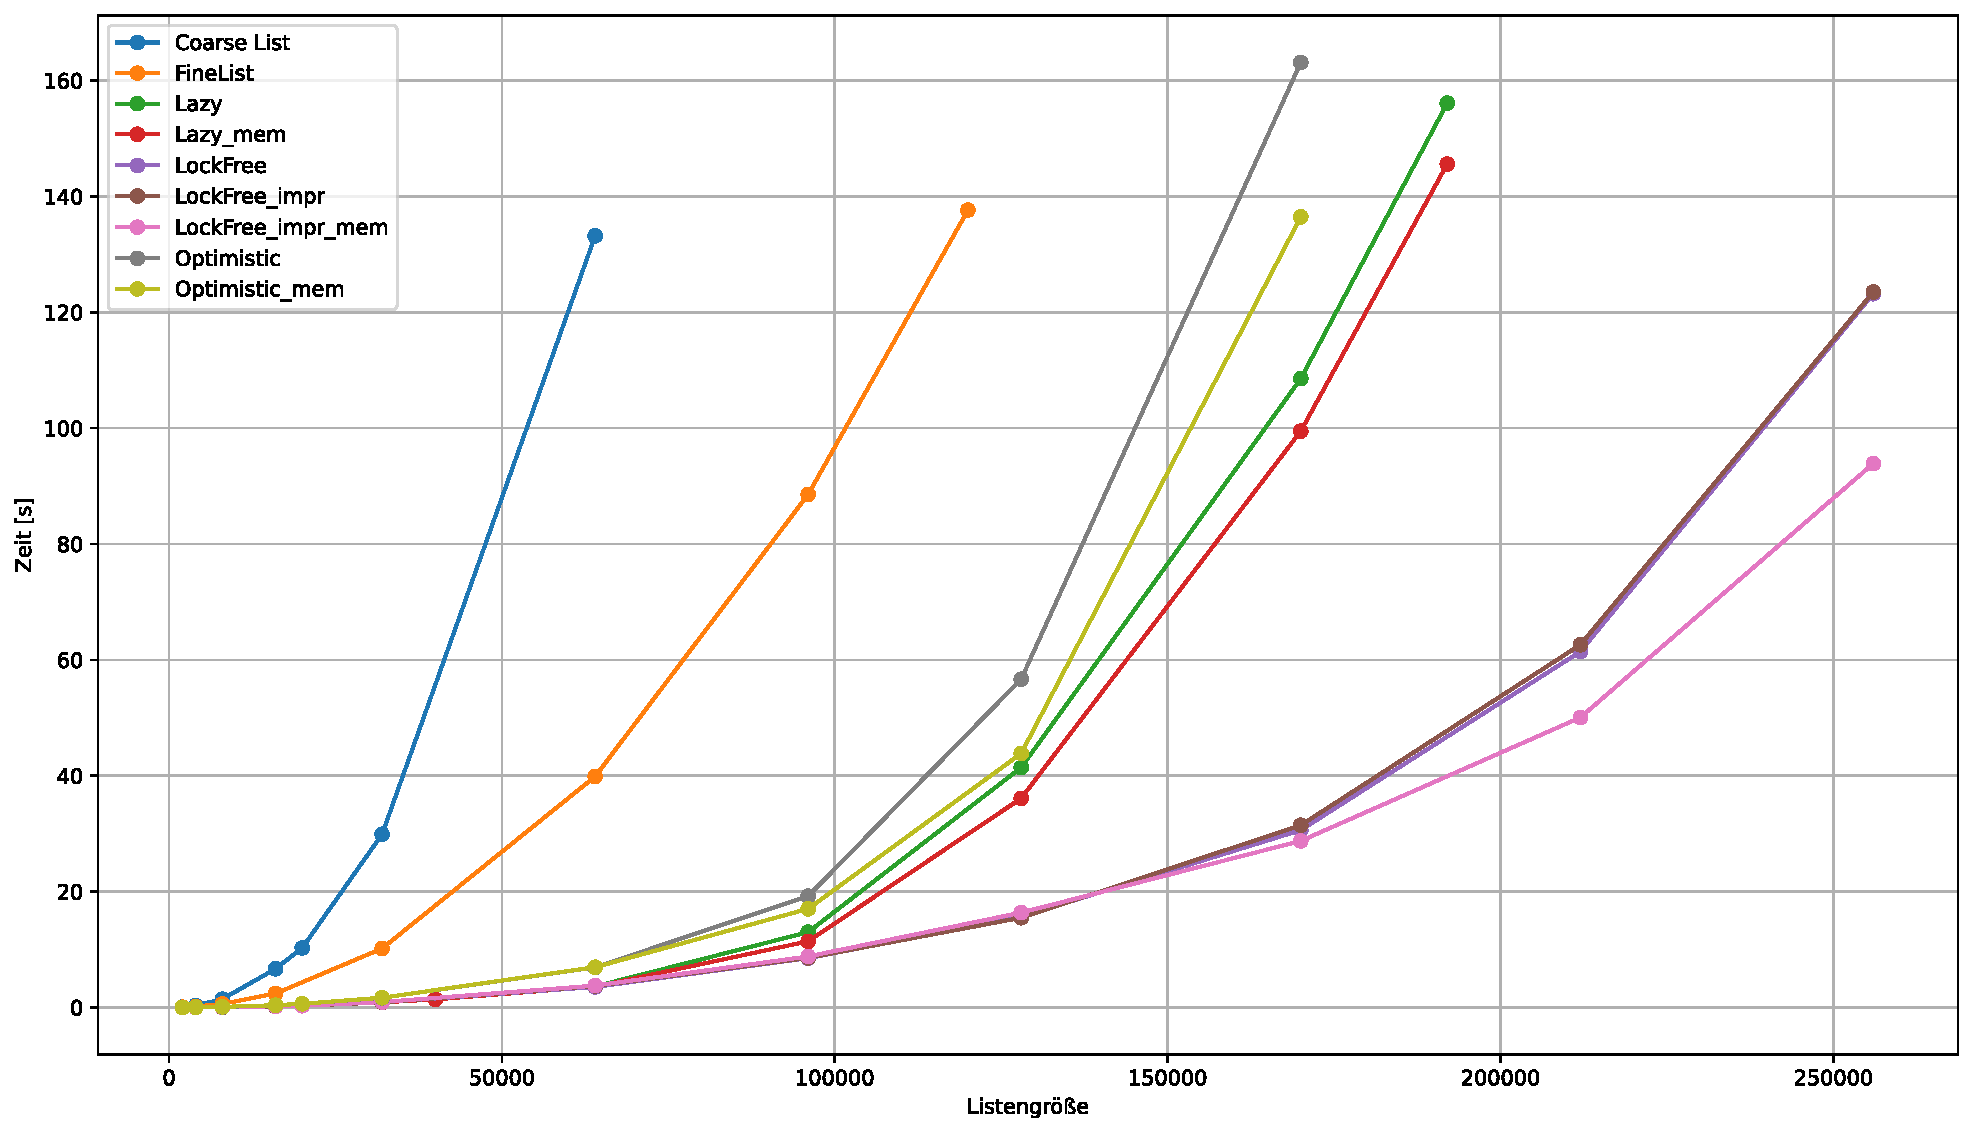
\includegraphics[width=1.0\linewidth]{./plots_pdf/mixed_time} 
	\caption{Laufzeit bei gemischten Zugriff}
	\label{fig:mixed_time} 
\end{figure}
Die Abbildung \ref{fig:write_time} zeigt die benötigte Laufzeit bei gemischten Zugriff. Dabei sind die Zugriffe folgendermaßen aufgeteilt:
 $50\%$ \textit{contain()}, $25\%$ \textit{add()} und $25\%$ \textit{remove()}.
 Dabei ist auf der X-Achse die größe der Liste zu sehen, was auch jeweils der Anzahl der hinzugefügten und entfernten Daten entspricht. 
 Auffallend ist hier, dass Datenstrukturen mit einen implementierten Memorymanagement bei großen Listen schneller sind, obwohl
 das Memorymanagement zusätzlichen aufwand bedeutet. Eine mögliche Begründung liegt darin, dass dem Betriebssystem immer wieder 
 Speicher zurückgegeben wird und somit das auslagern von Daten aus dem Cache minimiert wird.

\subsubsection{Lesender Zugriff}
\begin{figure}[ht!]
	\centering
	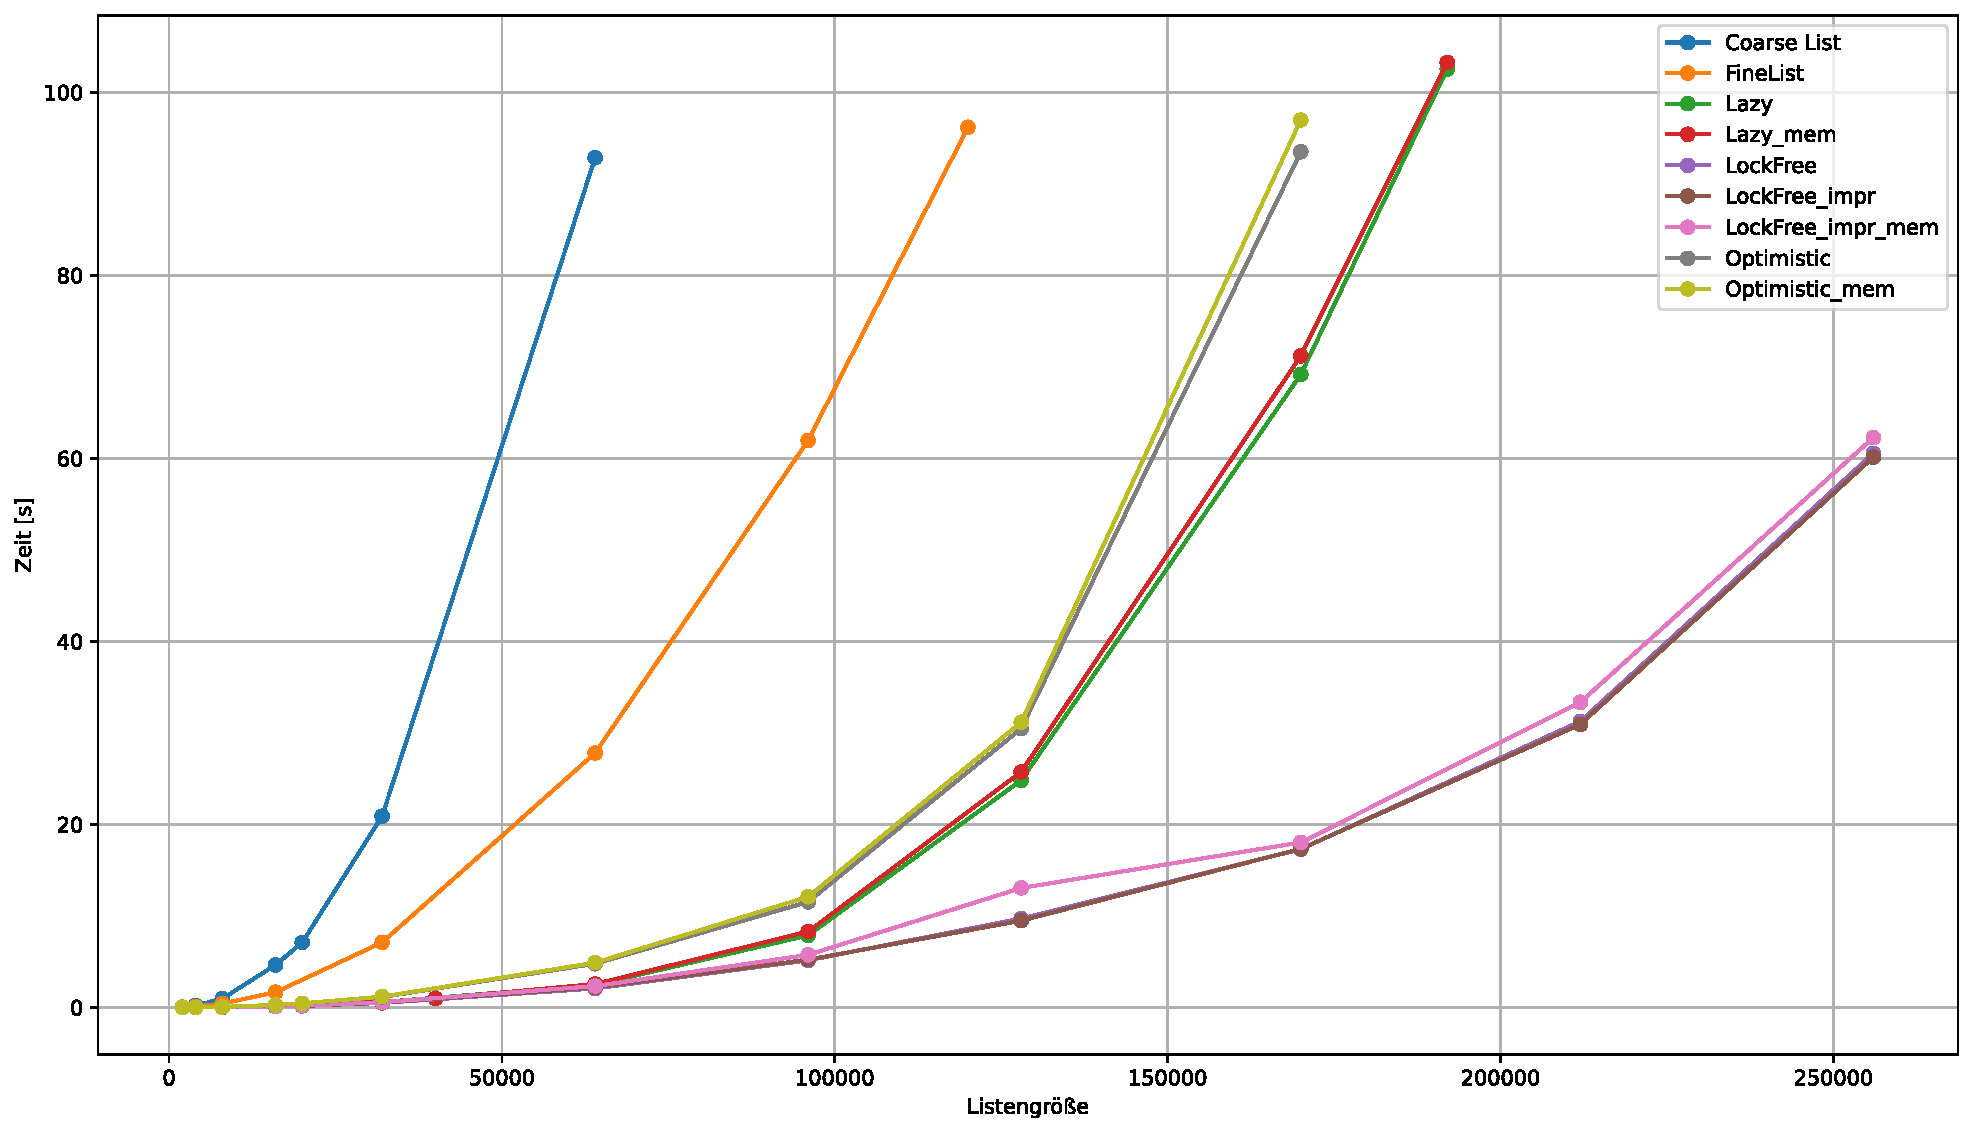
\includegraphics[width=1.0\linewidth]{./plots_pdf/check_time} 
	\caption{Laufzeit für Lesevorgang}
	\label{fig:check_time} 
\end{figure}
Die Abbildung \ref{fig:check_time} zeigt die benötigte Laufzeit, wenn auf die Datenstruktur nur mit \textit{contain()} zugegriffen wird.
Dabei wurden alle Listenelemente abgefragt. Desweiteren wurde die selbe Anzahl an Daten abgefragt, welche sich nicht in der Datenstruktur befinden.
Somit wurden doppelt so viel \textit{contain()} Anfragen ausgeführt, wie Listenelemente vorhanden sind.
Auffallend ist hier, dass beispielsweise die Lazy-Liste bei großen Listen erheblich länger benötigt, als die Lock-free list, obwohl die
\textit{contain()} identisch fast identisch sind. Eine mögliche Ursache ist die unterschiedliche größe der Nodes. Die Lazy.Liste beinhaltet
in ihren Nodes zusätzlich eine Variable für Mutex und einen Boolean zum markieren. Dieser Größenunterschied könnte für das
Memorymanagement des Betriebssystem einen erhöhten aufwand beim laden der Nodes beim durchlaufen bedeuten. Dies konnte jedoch eine Vermutung
und konnte nicht bestätigt werden.


\subsection{Neustarts von Zugriffen}
Wie bereits in Kapitel \ref{subsec:impr} beschrieben, kann es vorkommen, dass Datenstrukturen aufgrund eines konfliktes mit einem anderen
Thread einen laufenden Task neu beginnen müssen. 
In Abbildung \ref{fig:mixed_lostTime} ist zu sehen, wie oft eine laufende Funktion abgebrochen werden musste und wieder beim Listenkopf beginnen musste. 
In Abbildung \ref{fig:mixed_goToStart} ist ersichtlich, wie viel Zeit für diese Neustarts aufgewendet werden musste. \\
Bei einer Listengröße von 256000 mit 64 Cores und 512000 Zugriffen abfragen startet die Lock-free Liste 3163 mal neu. Dies bedeutet
einen zusätzlichen Zeitaufwand von 21 Sekunden. Somit spendet jeder Core 0,33 Sekunden mit Neustarts. Bei einer Laufzeit von 123204 Sekunden 
entspricht das 0,00028\% der Laufzeit. Da wie in Abbildung \ref{fig:mixed_lostTime} ersichtlich, steigt die zusätzliche Zeit durch Neustart exponentiell.
Somit wird dies bei noch größeren Listen relevant. Im zuge dieses Projektes wurden jedoch keine größeren Listen getestet. 

\begin{figure}[ht!]
	\centering
	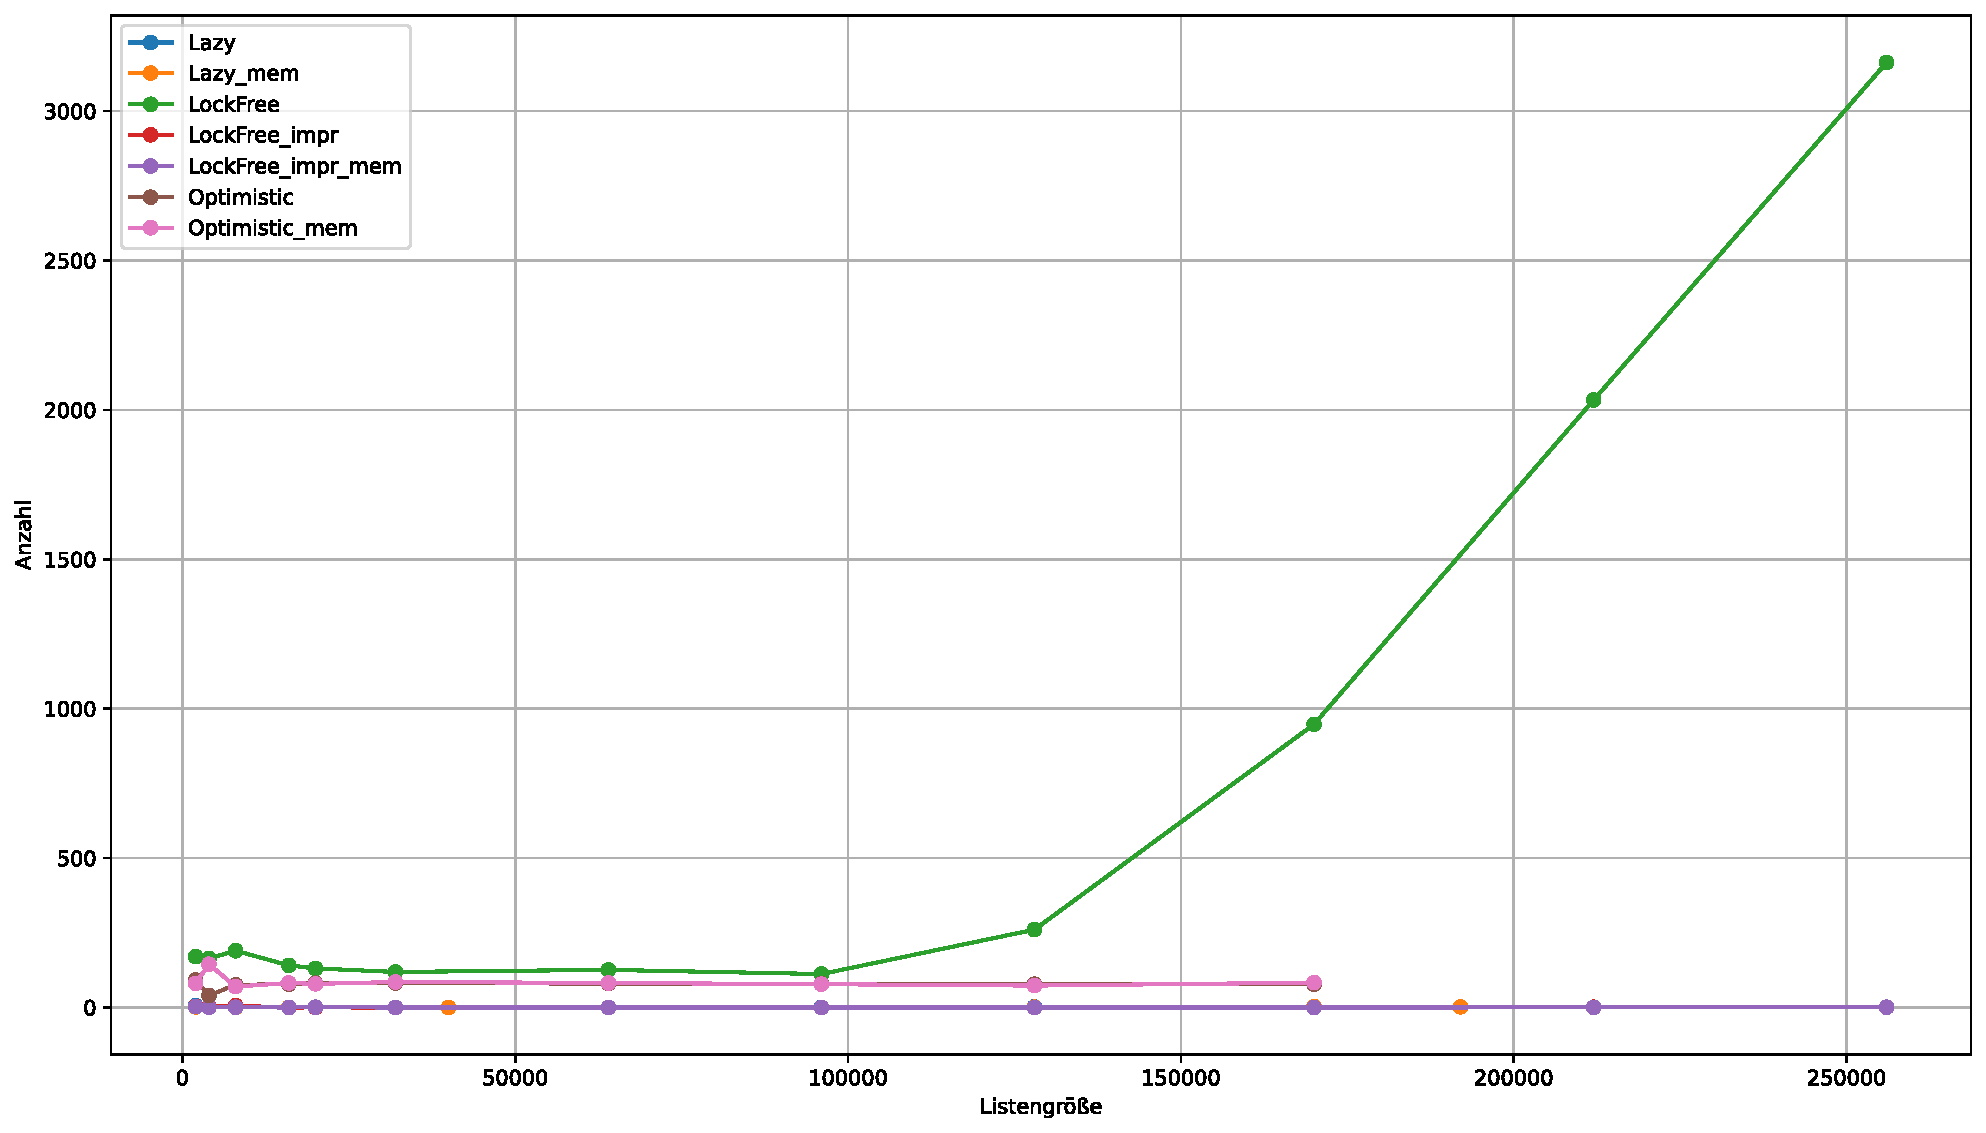
\includegraphics[width=1.0\linewidth]{./plots_pdf/mixed_goToStart.pdf} 
	\caption{Neustarts}
	\label{fig:mixed_goToStart} 
\end{figure}

\begin{figure}[ht!]
	\centering
	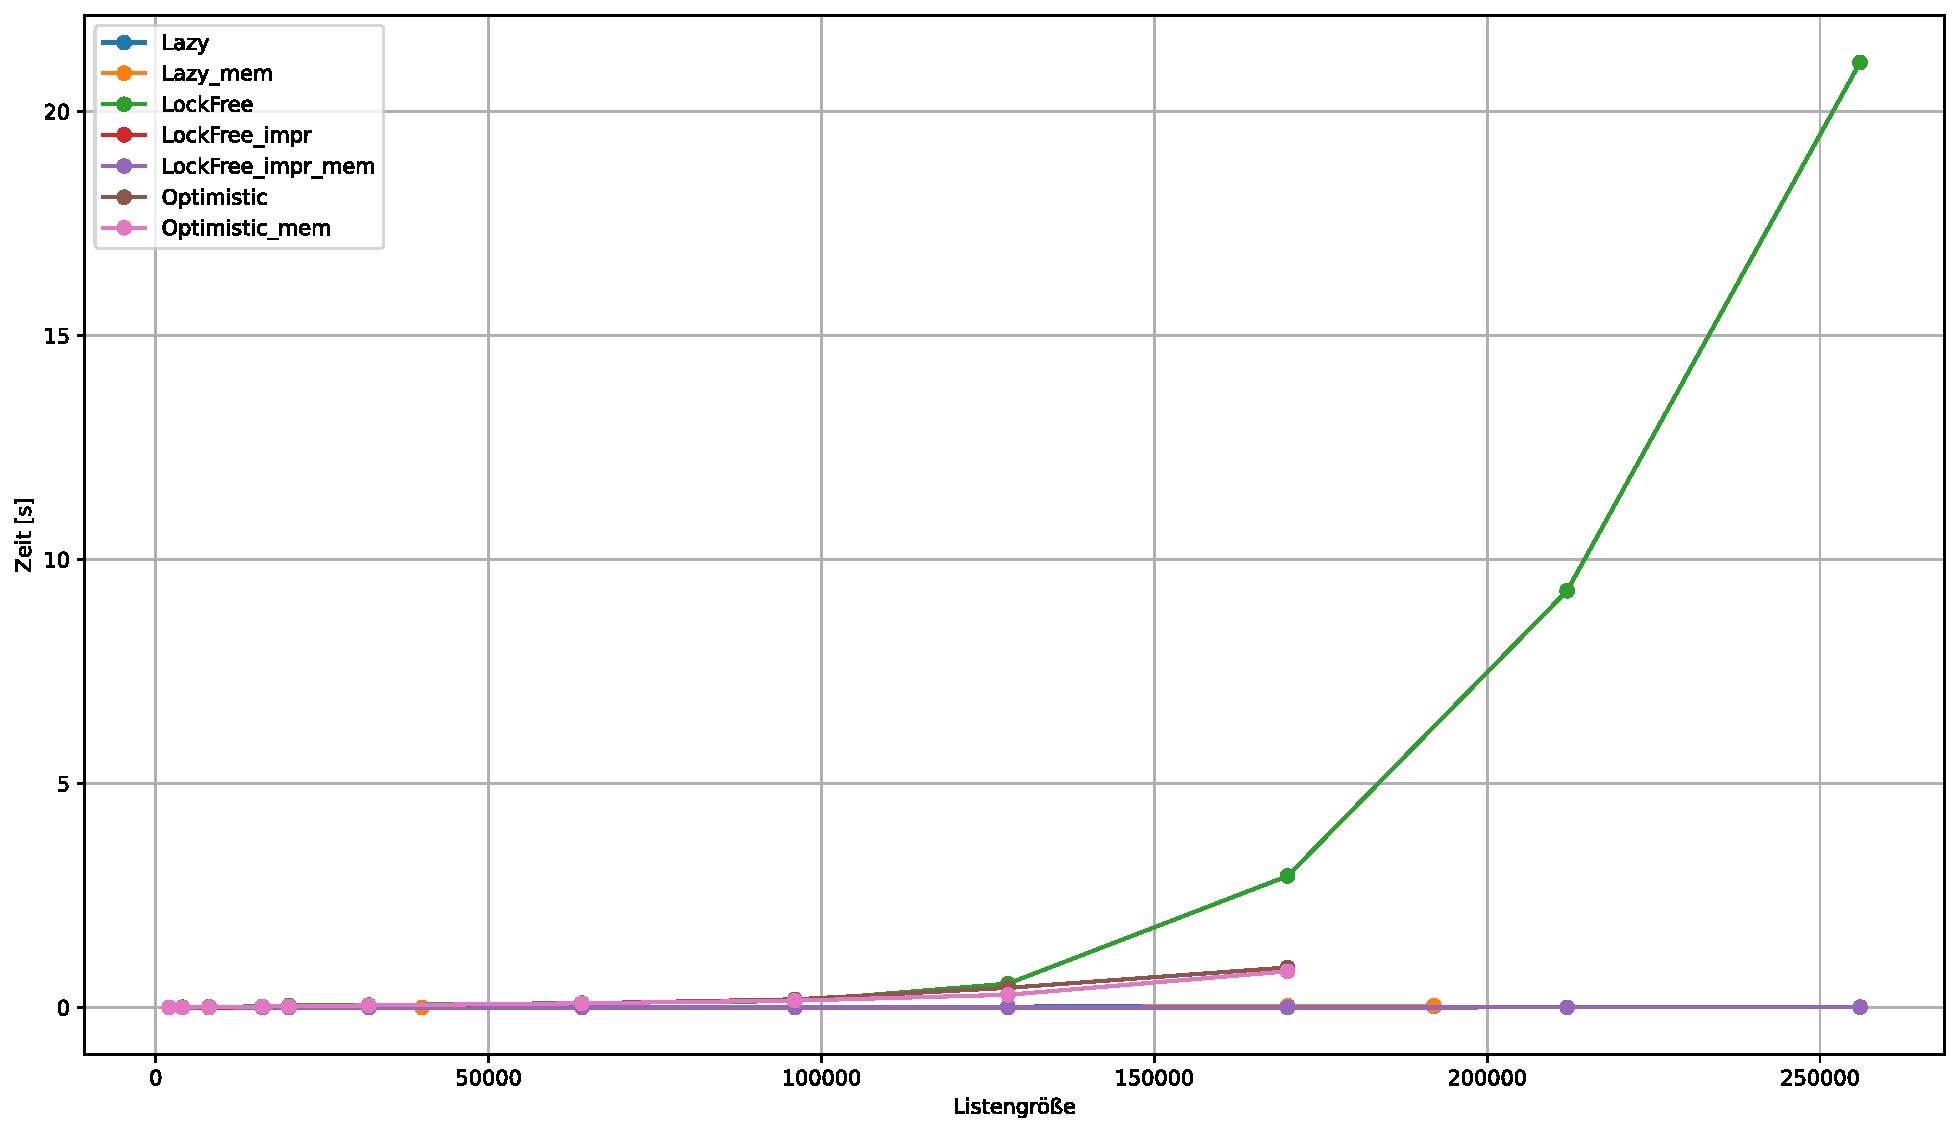
\includegraphics[width=1.0\linewidth]{./plots_pdf/mixed_lostTime.pdf} 
	\caption{Zusätzliche Zeit durch Neustarts}
	\label{fig:mixed_lostTime} 
\end{figure}

\subsection{Laufzeit mit unterschiedlichen Cores}